%%%%%%%%%%%%%%%%%%%%%%%%%%%%%%%%%%%%%%%%%
% Beamer Presentation
% LaTeX Template
% Version 1.0 (10/11/12)
%
% This template has been downloaded from:
% http://www.LaTeXTemplates.com
%
% License:
% CC BY-NC-SA 3.0 (http://creativecommons.org/licenses/by-nc-sa/3.0/)
%
%%%%%%%%%%%%%%%%%%%%%%%%%%%%%%%%%%%%%%%%%

%----------------------------------------------------------------------------------------
%	PACKAGES AND THEMES
%----------------------------------------------------------------------------------------

\documentclass{beamer}

\mode<presentation> {

% The Beamer class comes with a number of default slide themes
% which change the colors and layouts of slides. Below this is a list
% of all the themes, uncomment each in turn to see what they look like.

%\usetheme{default}
%\usetheme{AnnArbor}
%\usetheme{Antibes}
%\usetheme{Bergen}
%\usetheme{Berkeley}
%\usetheme{Berlin}
%\usetheme{Boadilla}
%\usetheme{CambridgeUS}
%\usetheme{Copenhagen} --
%\usetheme{Darmstadt} --
%\usetheme{Dresden}
%\usetheme{Frankfurt} --
%\usetheme{Goettingen}
%\usetheme{Hannover}
%\usetheme{Ilmenau}
%\usetheme{JuanLesPins}
%\usetheme{Luebeck}
\usetheme{Madrid}
%\usetheme{Malmoe}
%\usetheme{Marburg}
%\usetheme{Montpellier}
%\usetheme{PaloAlto}
%\usetheme{Pittsburgh}
%\usetheme{Rochester}
%\usetheme{Singapore}
%\usetheme{Szeged}
%\usetheme{Warsaw}

% As well as themes, the Beamer class has a number of color themes
% for any slide theme. Uncomment each of these in turn to see how it
% changes the colors of your current slide theme.

%\usecolortheme{albatross}
%\usecolortheme{beaver}
%\usecolortheme{beetle}
%\usecolortheme{crane}
%\usecolortheme{dolphin}
%\usecolortheme{dove}
%\usecolortheme{fly}
%\usecolortheme{lily}
%\usecolortheme{orchid}
%\usecolortheme{rose}
%\usecolortheme{seagull}
%\usecolortheme{seahorse}
%\usecolortheme{whale}
%\usecolortheme{wolverine}

%\setbeamertemplate{footline} % To remove the footer line in all slides uncomment this line
%\setbeamertemplate{footline}[page number] % To replace the footer line in all slides with a simple slide count uncomment this line

%\setbeamertemplate{navigation symbols}{} % To remove the navigation symbols from the bottom of all slides uncomment this line
}

\usepackage[spanish]{babel}
\usepackage[utf8]{inputenc}

\usepackage{graphicx} % Allows including images
\usepackage{booktabs} % Allows the use of \toprule, \midrule and \bottomrule in tables

\renewcommand\footnotemark{}
\renewcommand\footnoterule{}

%----------------------------------------------------------------------------------------
%	TITLE PAGE
%----------------------------------------------------------------------------------------

\title[RRAP]{Proyecto de grado: Routers Reconfigurables de Altas Prestaciones} % The short title appears at the bottom of every slide, the full title is only on the title page

\author{Rodrigo Amaro, Emiliano Viotti}
\institute[UdelaR] % Your institution as it will appear on the bottom of every slide, may be shorthand to save space
{
Instituto de Computaci\'on \\ Facultad de Ingeniería \\ Universidad de la República \\ \vspace{0.2cm} Tutores: Dr. Eduardo Gramp\'in, MSc. Mart\'in Giachino % Your institution for the title page
%\medskip
%\textit{john@smith.com} % Your email address
}
\date{\today} % Date, can be changed to a custom date

\begin{document}

\begin{frame}
\titlepage % Print the title page as the first slide
\end{frame}


\begin{frame}
\frametitle{Agenda} % Table of contents slide, comment this block out to remove it
\tableofcontents % Throughout your presentation, if you choose to use \section{} and \subsection{} commands, these will automatically be printed on this slide as an overview of your presentation
\end{frame}

%----------------------------------------------------------------------------------------
%	PRESENTATION SLIDES
%----------------------------------------------------------------------------------------

%------------------------------------------------
\begin{frame}
\frametitle{Motivaci\'on} 

\begin{block}{Redes acad\'emicas}
Internet no parece apropiada para su utilizaci\'on en el contexto académico en el desarrollo de nuevos protocolos y servicios, investigaci\'on y la innovaci\'on en el \'area.
\end{block}

\begin{figure}[h] 
\centering    
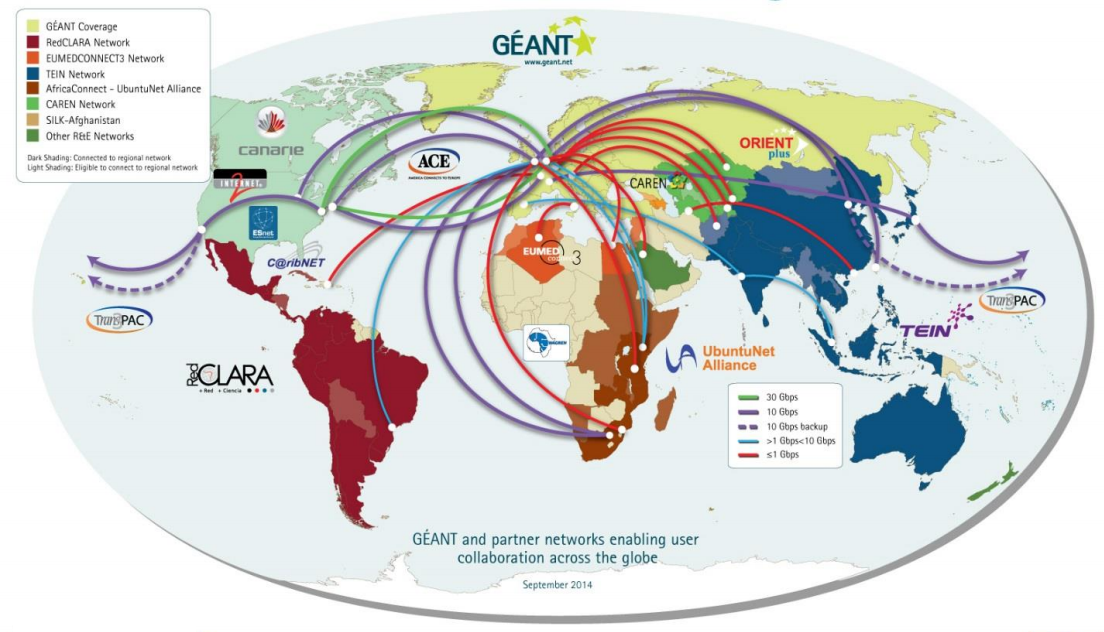
\includegraphics[width=0.7\textwidth]{imagenes/redesAcademicas.png}
\label{fig:4DProject}
\end{figure}

\end{frame}

\begin{frame}
\frametitle{Motivaci\'on} 

\begin{block}{Red Académica Uruguaya (RAU)}
A nivel local, la RAU es un emprendimiento de la Universidad de la República administrado por el SeCIU con los objetivos de unir a las instituciones académicas nacionales en una red de alcance nacional y a trav\'es de ella conectarlas a Latinoam\'erica. 
\end{block}

\begin{block}{RAU2}
Remplazo de la actual red académica, es una red avanzada de altas prestaciones que estar\'ia dotada de funciones de virtualizaci\'on de redes flexibles en su definici\'on y uso.
\end{block}

\begin{figure}[h] 
\centering    

\includegraphics[width=0.3\textwidth]{imagenes/logorau2.png}
\label{fig:4DProject}
\end{figure}

\end{frame}

\begin{frame}
\frametitle{Motivaci\'on} 

\begin{block}{Desarrollo e innovacion en el area}
Los equipos de red de backbone comerciales son caros y limitados a las funcionalidades de una API generalmente propietaria.
\end{block}
\end{frame}
%------------------------------------------------

%------------------------------------------------
\section{Conceptos preliminares} 
%------------------------------------------------

\begin{frame}
\frametitle{SDN} 

\end{frame}

\begin{frame}
\frametitle{OpenFlow} 

\end{frame}

\begin{frame}
\frametitle{VPN} 

\end{frame}

\begin{frame}
\frametitle{MPLS} 

\end{frame}

%------------------------------------------------
\section{Arquitectura de la soluci\'on} 

\begin{frame}
\frametitle{Arquitectura de la soluci\'on} 

\end{frame}
%------------------------------------------------

%------------------------------------------------
\section{Implementaci\'on} 

\begin{frame}
\frametitle{Implementaci\'on} 

\end{frame}
%------------------------------------------------

%------------------------------------------------
\section{Conclusiones} 

\begin{frame}
\frametitle{Conclusiones} 

\end{frame}
%------------------------------------------------

%------------------------------------------------
\section{Trabajo a futuro} 

\begin{frame}
\frametitle{Trabajo a futuro} 

\end{frame}
%------------------------------------------------

%----------------------------------------------------------------------------------------

\end{document} 
